\documentclass[UTF8,oneside]{ctexbook}

\usepackage[titles]{tocloft} % 目录
%\usepackage{graphicx} % An example of a floating figure using the graphicx package.
\usepackage{animate} % 动画
\usepackage[caption=true, font=footnotesize]{subfig}% 前面的[]为了防止覆盖IEEE默认选项
\usepackage{float} %禁止浮动
\usepackage{enumerate} % 列表
\usepackage{amsmath} % 数学
\usepackage{listings} %抄录环境
\usepackage{color} %定义颜色
\definecolor{codegreen}{rgb}{0,0.6,0}
\definecolor{codegray}{rgb}{0.5,0.5,0.5}
\definecolor{codepurple}{rgb}{0.58,0,0.82}
\definecolor{backcolour}{rgb}{0.95,0.95,0.92}

\definecolor{commentcolor}{rgb}{0.85, 0.85, 0.85}
\definecolor{keywordcolor}{rgb}{0.067, 0.004, 1}
\definecolor{stringcolor}{rgb}{0,0.6,0}
\definecolor{packagecolor}{rgb}{0,0.6,0}
\definecolor{envicolor}{rgb}{0,0.6,0}
%--------- 定义代码抄录格式 -------
\lstdefinestyle{myLaTeX}{
	language={[LaTeX]TeX},
	basicstyle=\small\ttfamily,
	backgroundcolor=\color{backcolour},
	commentstyle=\color{codegreen},
	keywordstyle=\color{magenta},
	numberstyle=\tiny\color{codegray},
	stringstyle=\color{codepurple},
	basicstyle=\footnotesize,
	%
	breakatwhitespace=false,
	breaklines=true, % 允许断行                 
	captionpos=b,
	keepspaces=true,
	numbers=none,numbersep=5pt,
	showspaces=false,
	showstringspaces=false,
	showtabs=false,
	tabsize=2,
	%
	classoffset=1,morekeywords={ctexbook},keywordstyle=\color{keywordcolor}, % classoffest=0为更改默认值
}
\usepackage[colorlinks,linkcolor=blue]{hyperref} % 超链接
\usepackage[margin=3cm]{geometry} % 更改页边距

\usepackage{tcolorbox} % 用于生成彩色文本框
\tcbuselibrary{listings,skins,breakable} %调用程序库
\newtcblisting{mybox}[2][]{colback=black!10!white,colframe=blue!75!black,fonttitle=\bfseries,title=#2,#1,breakable,bicolor,colbacklower=white,% 运行结果部分颜色
interior style={left color=yellow!90,right color=green!40},
frame style={left color=red!75!black,right color=blue!75!black},%哪个[]里有数,证明哪个是必填参数
listing options={
	style=tcblatex,keywordstyle=\color{blue},commentstyle=\color{green!50!black},numbers=none,numberstyle=\tiny\color{red!75!black}\emptyaccsupp,emptylines=1,escapeinside=
	}
}
\usepackage{booktabs} % 用于生成三线表
\usepackage{multirow} % 多行
\usepackage{array}






\title{{C4D简明教程}\\
\large{V1.0}}
\author{\href{https://github.com/lonelybag?tab=repositories}{\itshape{@LonelyBag}}\\ {\itshape \large{Edite by \href{https://mirrors.tuna.tsinghua.edu.cn/CTAN/systems/texlive/Images/}{\LaTeX}}}}

\begin{document}
% ----------- 封面 ---------------
\frontmatter
\maketitle
% ----------- 目录 ---------------
\tableofcontents
\mainmatter
% ----------- 正文 ---------------
\chapter{基本操作}
\begin{itemize}
    \item 更改分辨率:打开渲染器设置,Ctrl + B
    \item 旋转视图:按住Alt + 鼠标
    \item 新建材质:双击材质栏
    \item 新增材料属性:双击材质球
    \item 赋予材料:将材质球拖放至几何体上
    \item 旋转:R键
    \item 缩放:T键
    \item 按住Shift调节,以10为单位
    \item 按住Alt调节,以0.1位单位
    \item 单击右键,复位
    \item 线条着色:N + B
    \item 连接对象并删除
    \item 按住ctrl键进行选择是消除
    \item 按住ctrl键拖拽中键是改变选择范围
    \item 循环选择,选择一圈点,U + L
    \item 按住ctrl进行拖拽
    \item 内部挤压,i键
    \item 挤压,D键
    \item 切刀工具,k键,在平面视图操作
    \item 两个面相接的地方如果点没有相连,那么需要优化
    \item 焊接两个点,M-Q
    \item 断开一条线,先切刀,然后右键选择断开连接
    \item 调用弹出菜单,V
    \item 显示材质颜色,点击shift+V,查看-纹理
    \item 删除多余点,选中-消除
    \item 
\end{itemize}
\chapter{使用场景}
\section{插入背景图}
\begin{itemize}
    \item 将视图转换为平面视图,比如:正视图
    \item 打开视窗属性:Shift + V
    \item 点击按钮选择图片
    \begin{figure}[H]
        \centering
        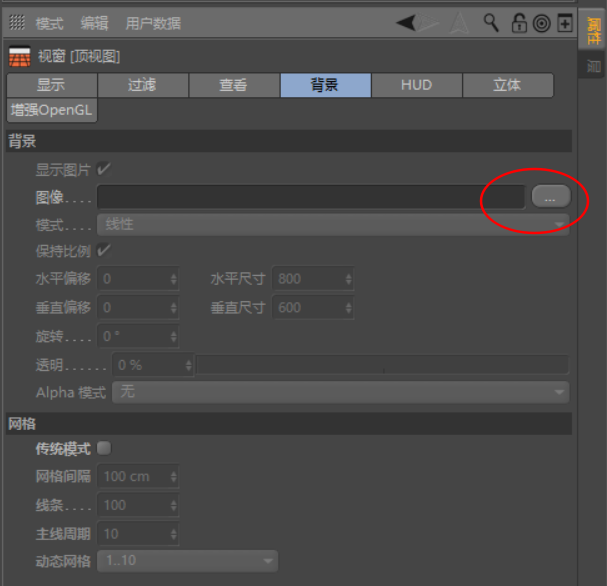
\includegraphics[width=0.5\linewidth]{Fig//put_fig.png}
        \vspace{-0.3cm}
        \caption{选择图片}\label{fig:put_fig}
    \end{figure}
    \item 调节透明度、尺寸等
    \begin{figure}[H]
        \centering
        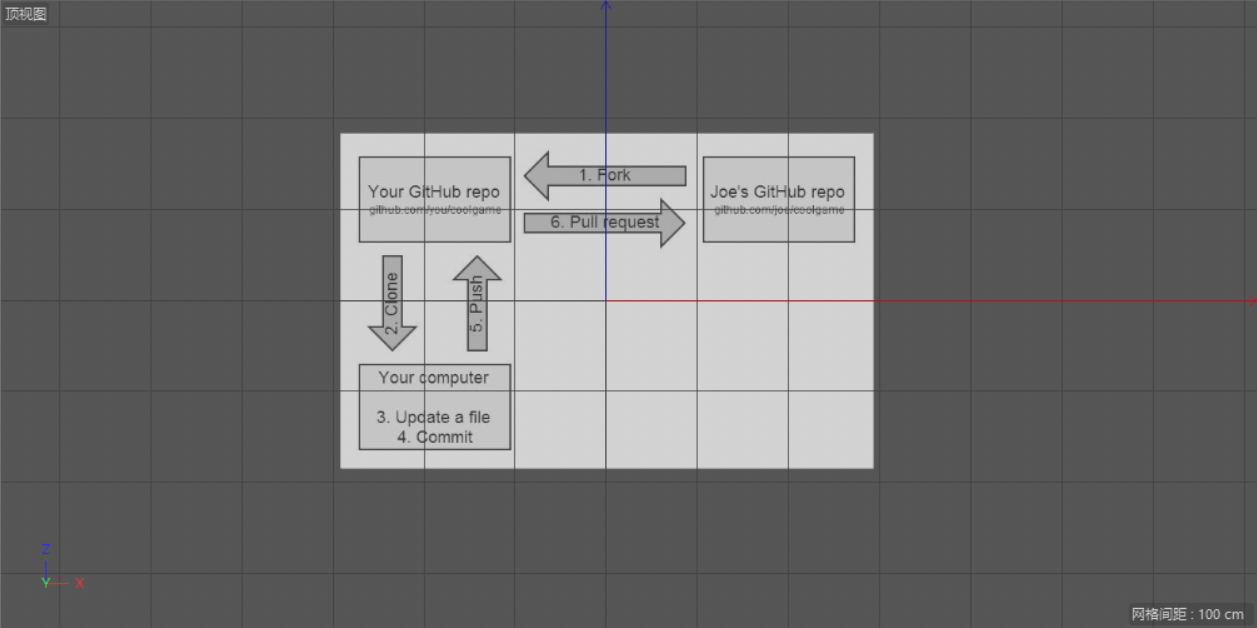
\includegraphics[width=0.5\linewidth]{Fig//put_fig_2.png}
        \vspace{-0.3cm}
        \caption{选择图片}\label{fig:put_fig_2}
    \end{figure}
\end{itemize}
\section{贴图}
\subsection{环境}
\begin{itemize}
    \item 添加材质
    \item 仅打开发光属性
    \begin{figure}[H]
        \centering
        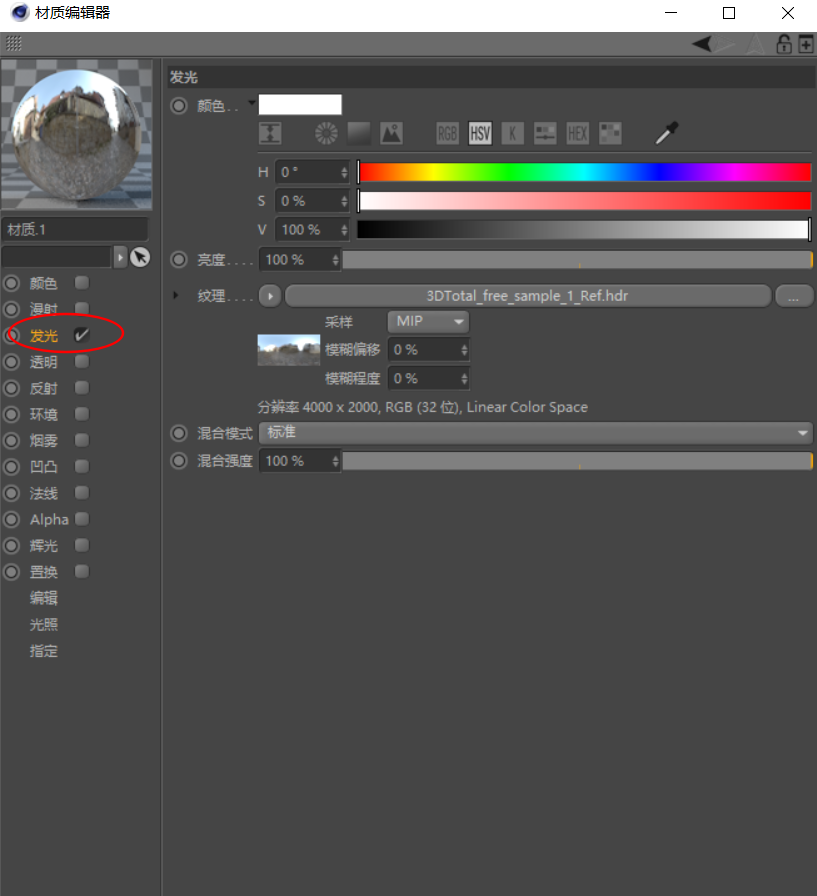
\includegraphics[width=0.5\linewidth]{Fig//envior_01.png}
        \vspace{-0.3cm}
        \caption{发光属性设置}\label{fig:envior_01}
    \end{figure}
    \item 窗口 - 内容贴图 - 拖拽到纹理
    \item 
\end{itemize}
\subsection{反射材质}
\begin{itemize}
    \item 添加颜色(是一种底色)
    \begin{figure}[H]
        \centering
        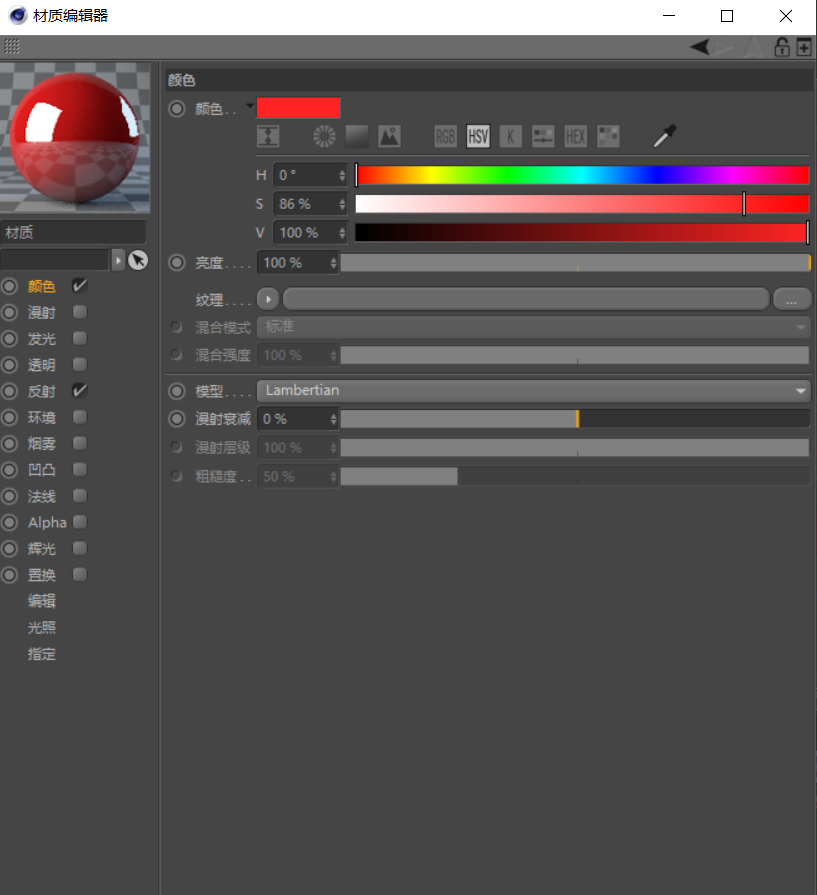
\includegraphics[width=0.5\linewidth]{Fig//ref_01.png}
        \vspace{-0.3cm}
        \caption{颜色属性}\label{fig:ref_01}
    \end{figure}
    \item 添加反射-层\footnote{注意,这里的层有先后顺序}
    \begin{figure}[H]
        \centering
        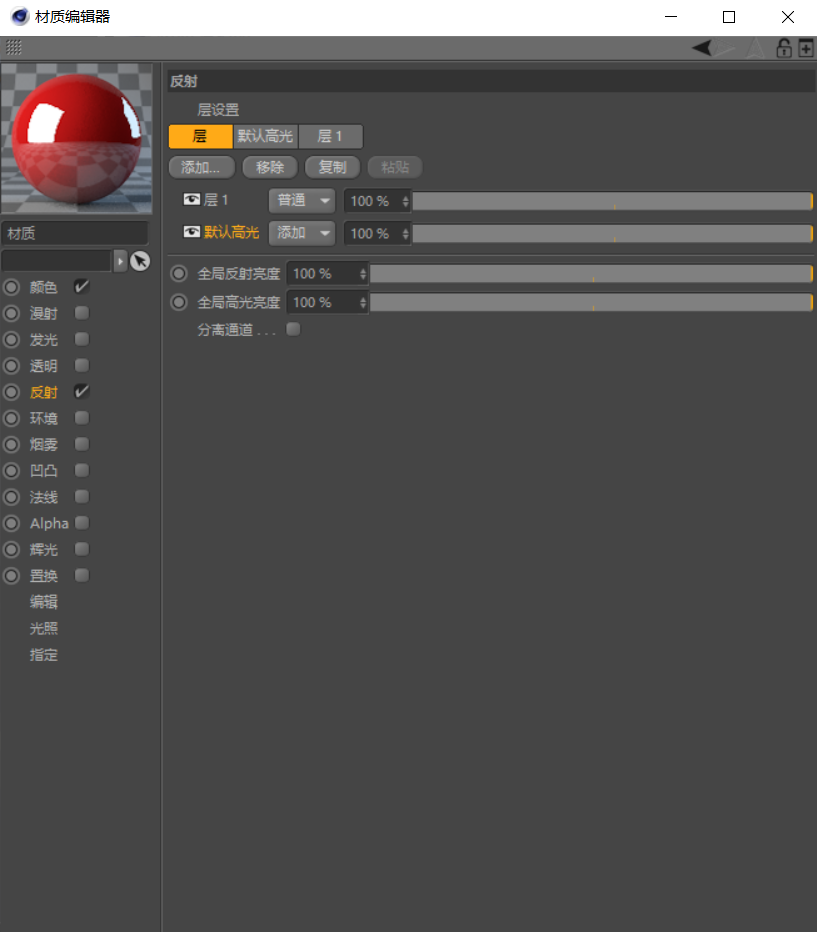
\includegraphics[width=0.5\linewidth]{Fig//ref_02.png}
        \vspace{-0.3cm}
        \caption{颜色属性}\label{fig:ref_02}
    \end{figure}
    \item 修改高光
    \begin{figure}[H]
        \centering
        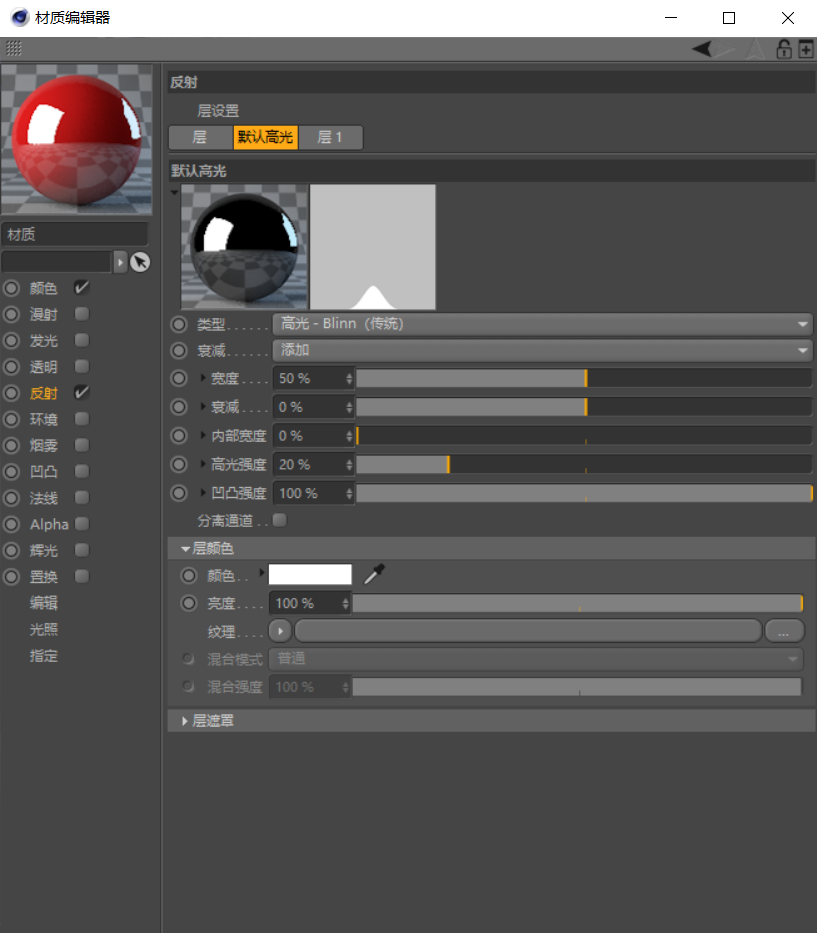
\includegraphics[width=0.5\linewidth]{Fig//ref_03.png}
        \vspace{-0.3cm}
        \caption{颜色属性}\label{fig:ref_03}
    \end{figure}
    \item 修改层
    \begin{figure}[H]
        \centering
        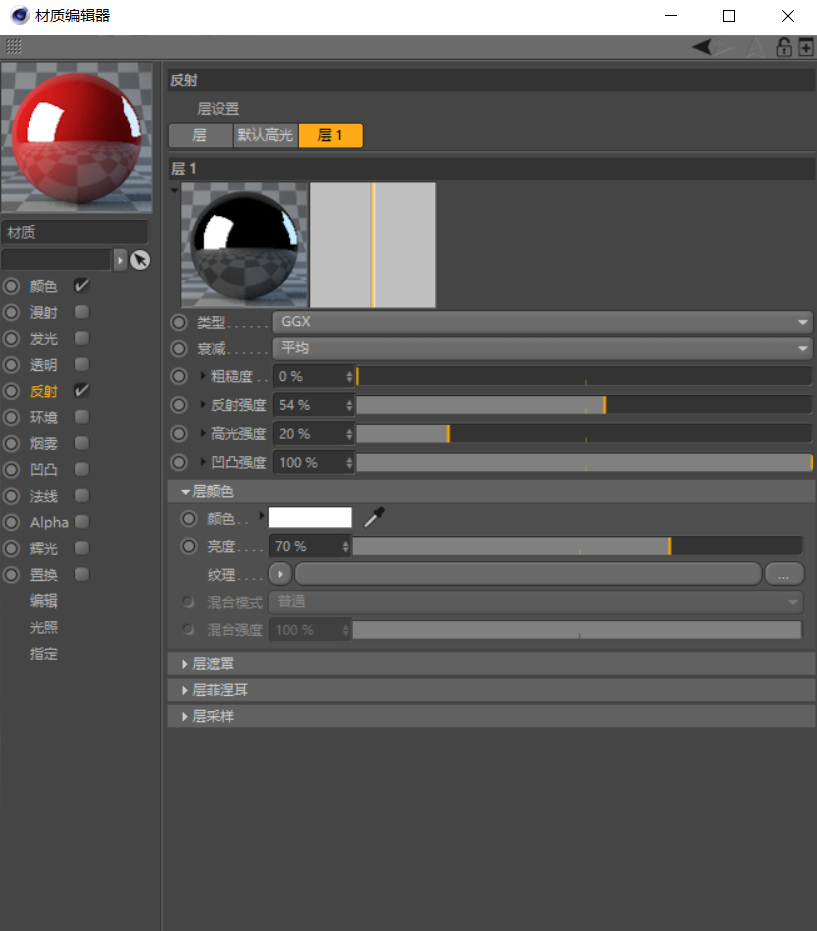
\includegraphics[width=0.5\linewidth]{Fig//ref_04.png}
        \vspace{-0.3cm}
        \caption{颜色属性}\label{fig:ref_04}
    \end{figure}
\end{itemize}
\begin{itemize}
    \item 层颜色控制反射与其它属性的颜色关系
    \item 
\end{itemize}
\section{渲染}
\begin{itemize}
    \item 快速渲染:Ctrl + R
    \item 区域渲染:Alt + R
    \item 渲染到图片查看器:Shift + R
\end{itemize}

\section{投影}
\begin{itemize}
    \item 添加灯光
    \item 投影 - 阴影贴图(软阴影)
\end{itemize}

\section{扫描}
注意:所有扫描对象必须为样条。
\begin{figure}[H]
	\centering
	\animategraphics[controls, loop , width=0.8\linewidth]{5}{Fig//sweep//}{1}{32}
	\vspace{-0.3cm}
	\caption{扫描}\label{fig:sweep}
\end{figure}

\end{document}